\section{One-at-a-time}
\subsection{Scenario 7}
This section discusses the results of the \gls{OAT} sensitivity analysis 
as applied to Scenario 7. A subsection of this analysis is presented 
in \hl{Cite ANS Paper}, but the analysis presented here has an expanded scope. 
Additionally, the work presented here uses an updated deployment scheme to 
account for non-consistent replacement of advanced reactors identified in 
\hl{ANS Paper}. The results discuss
the relative change in each metric for each parameter varied. The minimum, 
average, and maximum value for each metric is provided in Table 
\ref{tab:oat_values}.

\begin{table}
    \centering
    \caption{Minimum, average, and maximum value of each metric caused 
    by the variation of each parameter.}
    \label{tab:oat_values}
    \begin{tabular}{llrrr}       
        \hline 
        Parameter &     Metric &      Minimum &      Average &      Maximum \\\hline
        Transition Start &  Fuel Mass & 2.832004e+07 & 3.001442e+07 & 3.085691e+07 \\
                         & HALEU Mass & 2.777396e+07 & 2.931392e+07 & 3.005491e+07 \\ 
                         &  Total SWU & 9.727160e+08 & 1.035603e+09 & 1.067644e+09 \\ 
                         & HALEU SWU & 9.690305e+08 & 1.030876e+09 & 1.062295e+09 \\
                         &        SNF & 2.600173e+07 & 2.743657e+07 & 2.812741e+07 \\  
                         & HALEU Feed & 8.406729e+08 & 8.936249e+08 & 9.204018e+08 \\\hline
        LWR Lifetimes &  Fuel Mass & 2.226230e+07 & 2.574361e+07 & 2.933547e+07 \\
                      & HALEU Mass & 2.186991e+07 & 2.527842e+07 & 2.884623e+07 \\
                      &  Total SWU & 7.779876e+08 & 8.972582e+08 & 1.021053e+09 \\
                      &  HALEU SWU & 7.753394e+08 & 8.941187e+08 & 1.017751e+09 \\
                      &        SNF & 1.955625e+07 & 2.305043e+07 & 2.668538e+07 \\
                      & HALEU Feed & 6.715754e+08 & 7.746336e+08 & 8.819633e+08 \\\hline 
        Xe-100 Build Share &  Fuel Mass & 8.228834e+07 & 1.130189e+08 & 1.471439e+08 \\
                           & HALEU Mass & 2.826681e+06 & 1.077601e+07 & 1.803929e+07 \\
                           &  Total SWU & 1.082813e+09 & 1.089912e+09 & 1.101530e+09 \\
                           &  HALEU SWU & 1.275350e+08 & 3.998760e+08 & 6.501138e+08 \\
                           &        SNF & 7.510853e+07 & 1.032204e+08 & 1.344031e+08 \\
                           & HALEU Feed & 1.081440e+08 & 3.448436e+08 & 5.622094e+08 \\\hline 
        MMR Build Share &  Fuel Mass & 3.701890e+07 & 4.917833e+07 & 6.134049e+07 \\
                        & HALEU Mass & 2.670288e+07 & 3.851759e+07 & 5.039230e+07 \\
                        &  Total SWU & 9.901021e+08 & 1.599871e+09 & 2.211838e+09 \\
                        &  HALEU SWU & 9.204794e+08 & 1.527922e+09 & 2.137948e+09 \\
                        &        SNF & 3.439781e+07 & 4.065525e+07 & 4.688864e+07 \\
                        & HALEU Feed & 7.995188e+08 & 1.309634e+09 & 1.821949e+09 \\\hline 
        VOYGR Build Share &  Fuel Mass & 3.044985e+07 & 6.435525e+07 & 9.510189e+07 \\
                          & HALEU Mass & 1.515573e+07 & 2.233175e+07 & 3.044985e+07 \\
                          &  Total SWU & 1.076518e+09 & 1.082445e+09 & 1.092329e+09 \\
                          &  HALEU SWU & 5.527729e+08 & 7.988284e+08 & 1.079883e+09 \\
                          &        SNF & 2.764653e+07 & 5.870293e+07 & 8.679207e+07 \\
                          & HALEU Feed & 4.774801e+08 & 6.913159e+08 & 9.353306e+08 \\\hline 
        Xe-100 Burnup &  Fuel Mass & 2.760515e+07 & 5.887765e+07 & 1.591116e+08 \\
                      & HALEU Mass & 2.681265e+07 & 5.808515e+07 & 1.583191e+08 \\
                      &  Total SWU & 9.558796e+08 & 2.033879e+09 & 5.489061e+09 \\
                      &  HALEU SWU & 9.505310e+08 & 2.028530e+09 & 5.483713e+09 \\
                      &        SNF & 2.486320e+07 & 5.613569e+07 & 1.563697e+08 \\
                      & HALEU Feed & 8.233245e+08 & 1.759663e+09 & 4.760799e+09 \\\hline 
        MMR Burnup &  Fuel Mass & 3.064950e+07 & 3.123978e+07 & 3.292776e+07 \\
                   & HALEU Mass & 2.985700e+07 & 3.044728e+07 & 3.213526e+07 \\
                   &  Total SWU & 1.058714e+09 & 1.085347e+09 & 1.161506e+09 \\
                   &  HALEU SWU & 1.053366e+09 & 1.079998e+09 & 1.156157e+09 \\
                   &        SNF & 2.790754e+07 & 2.849783e+07 & 3.018581e+07 \\
                   & HALEU Feed & 9.128300e+08 & 9.354133e+08 & 9.999926e+08 \\
        \hline
    \end{tabular}
\end{table}


\subsubsection{Transition start time}
Delays in the transition start time generally decrease all of the output 
metrics, as shown in Figure \ref{fig:ts_scenario7}. This results matches 
expectations, because if the advanced reactors are deployed for less time, 
then they require fewer resources. However, there are some increases in 
the output metrics between individual time steps. For example, a transition 
start time of October 2029 increases the fuel mass and \gls{SNF} mass 
relative to July 2029. This increase is the result of changes in the number 
of each advanced reactor deployed, because of differences in the gap 
between energy produced and energy demand that must initially be filled when 
advanced reactors are deployed. By waiting until October 2029, more VOYGRs 
are deployed than when the transition starts in July 2029. As discussed in 
Chapter \ref{ch:once_through_results}, the VOYGR needs a larger fuel mass, 
and thus discharges more \gls{SNF} than the Xe-100 and \gls{MMR}. Therefore, 
these two metrics increase for this particular transition start time. 

\begin{figure}
    \centering
    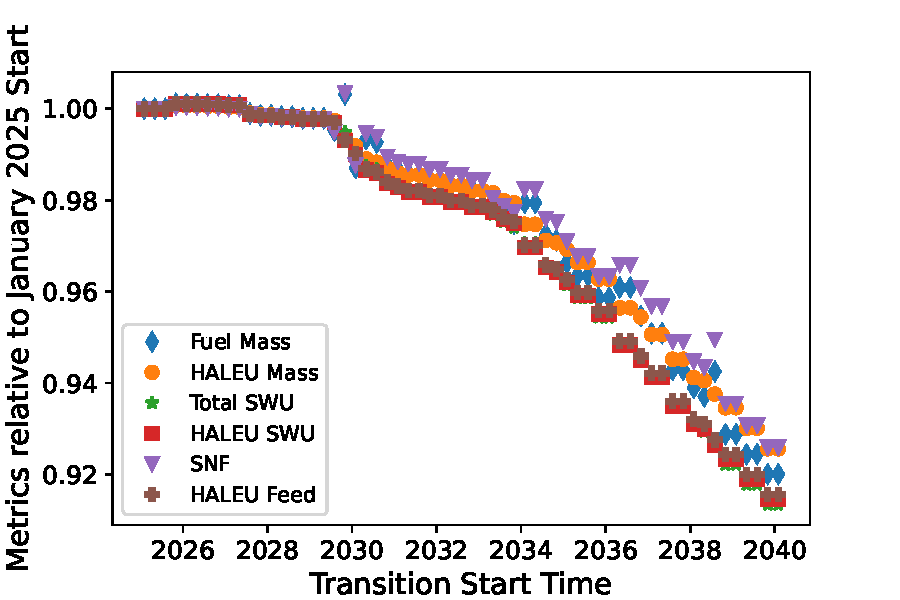
\includegraphics[scale=0.8]{ts.pdf}
    \caption{Change in each metric as a function of transition start 
    time, relative to a transition start in January 2025.}
    \label{fig:ts_scenario7}
\end{figure}

The \gls{HALEU} mass required for these transitions varied between 27.8-30.9
MTU. 

One of the disadvantages in delaying the transition start time is the 
increasing gap between energy supplied and energy demand as the transition 
start time is delayed. All of these scenarios have a constant demand 
of 87.20 GWe-yr beginning in 2025. By delaying the transition start time 
to after September 2025 (the observed initial deployment time of advanced 
reactors in Section \ref{sec:nogrowth_reactors}) there is some gap between 
the energy supplied and the energy demand. The largest gap observed is 36.7
GWe-yr, when reactors are deployed starting in January 2040. This difference 
between energy supplied and energy demand is a disadvantage of delaying 
the start time to reduce material requirements. 

\subsubsection{LWR lifetimes}
The next metric varied is the percent of the \glspl{LWR} that operate for 
80 years, reflecting a license extension. As the percent of the \gls{LWR} 
fleet operating for 80 years increases all of the metrics decrease, as 
Figure \ref{fig:lwr_scenario7} shows. All of the metrics decrease by a similar 
magnitude, with some variation because of changes in the number of each advanced 
reactor deployed, as previously discussed. The \gls{SNF} mass decreases more 
than the other metrics across this parameter space, ranging between 
19.5-26.7 MTU.

\begin{figure}
    \centering
    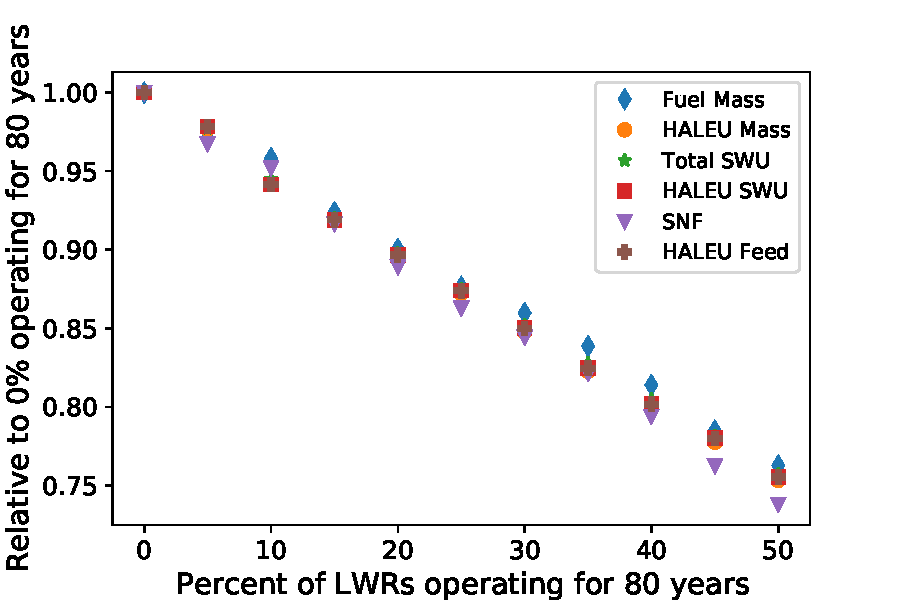
\includegraphics[scale=0.8]{lwr.pdf}
    \caption{Change in each metric as a function of percent of LWR fleet  
    operating for 80 years, relative to 0\%.}
    \label{fig:lwr_scenario7}
\end{figure}

Across this parameter space, the metrics decrease by a greater fraction than 
when varying the transition start time. The increased impact on the metrics 
is partly because the \glspl{LWR} that don't operate for 80 years all operate for 
60 years when varying this parameter, but not all of the \glspl{LWR} operate for 
60 years in the initial transition analysis or when varying the transition
start time. This modeling difference, made to simplify defining the advanced 
reactor deployment schedule, does not have a large impact on the results as 
evidenced by the maximum \gls{HALEU} mass when varying the \gls{LWR} lifetimes 
being only 4.9\% lower than the maximum \gls{HALEU} mass when varying the 
transition start time. This minimal impact from the modeling difference is 
because most of the \glspl{LWR} operate for 60 years when varying the transition start 
time. Therefore, we can attribute most of the change in the metrics to the 
change in the \gls{LWR} lifetimes. In addition to causing greater change in 
the metrics, the energy demand is always met when varying the \gls{LWR} lifetimes,
which suggests that extending the lifetimes of the \glspl{LWR} is a better 
parameter to vary if one wishes to decrease material requirements of this 
transition. 

\subsubsection{Xe-100 build share}
As the Xe-100 build share increases, the \gls{HALEU}-related metrics 
increase while the total \gls{SNF} and total fuel mass decrease and the 
total \gls{SWU} capacity stays relatively constant (Figure \ref{fig:xe100_scenario7}).
As Figure \ref{fig:xe100_s7_combined_reactors} shows, as the Xe-100 build share 
increases, the number of \glspl{MMR} is relatively constant and the number of 
VOYGRs decreases. These results show that as the Xe-100 build share increases, they 
are primarily replacing power that is supplied by the VOYGRs, instead of a portion 
of each of the other advanced reactors. This replacement of VOYGRs is because 
of the deployment scheme of this work, as the VOYGR has the largest power output 
between the VOYGR and \gls{MMR}. Therefore, the VOYGR is primarily deployed when 
the Xe-100 build share is 0\%. 

\begin{figure}
    \centering
    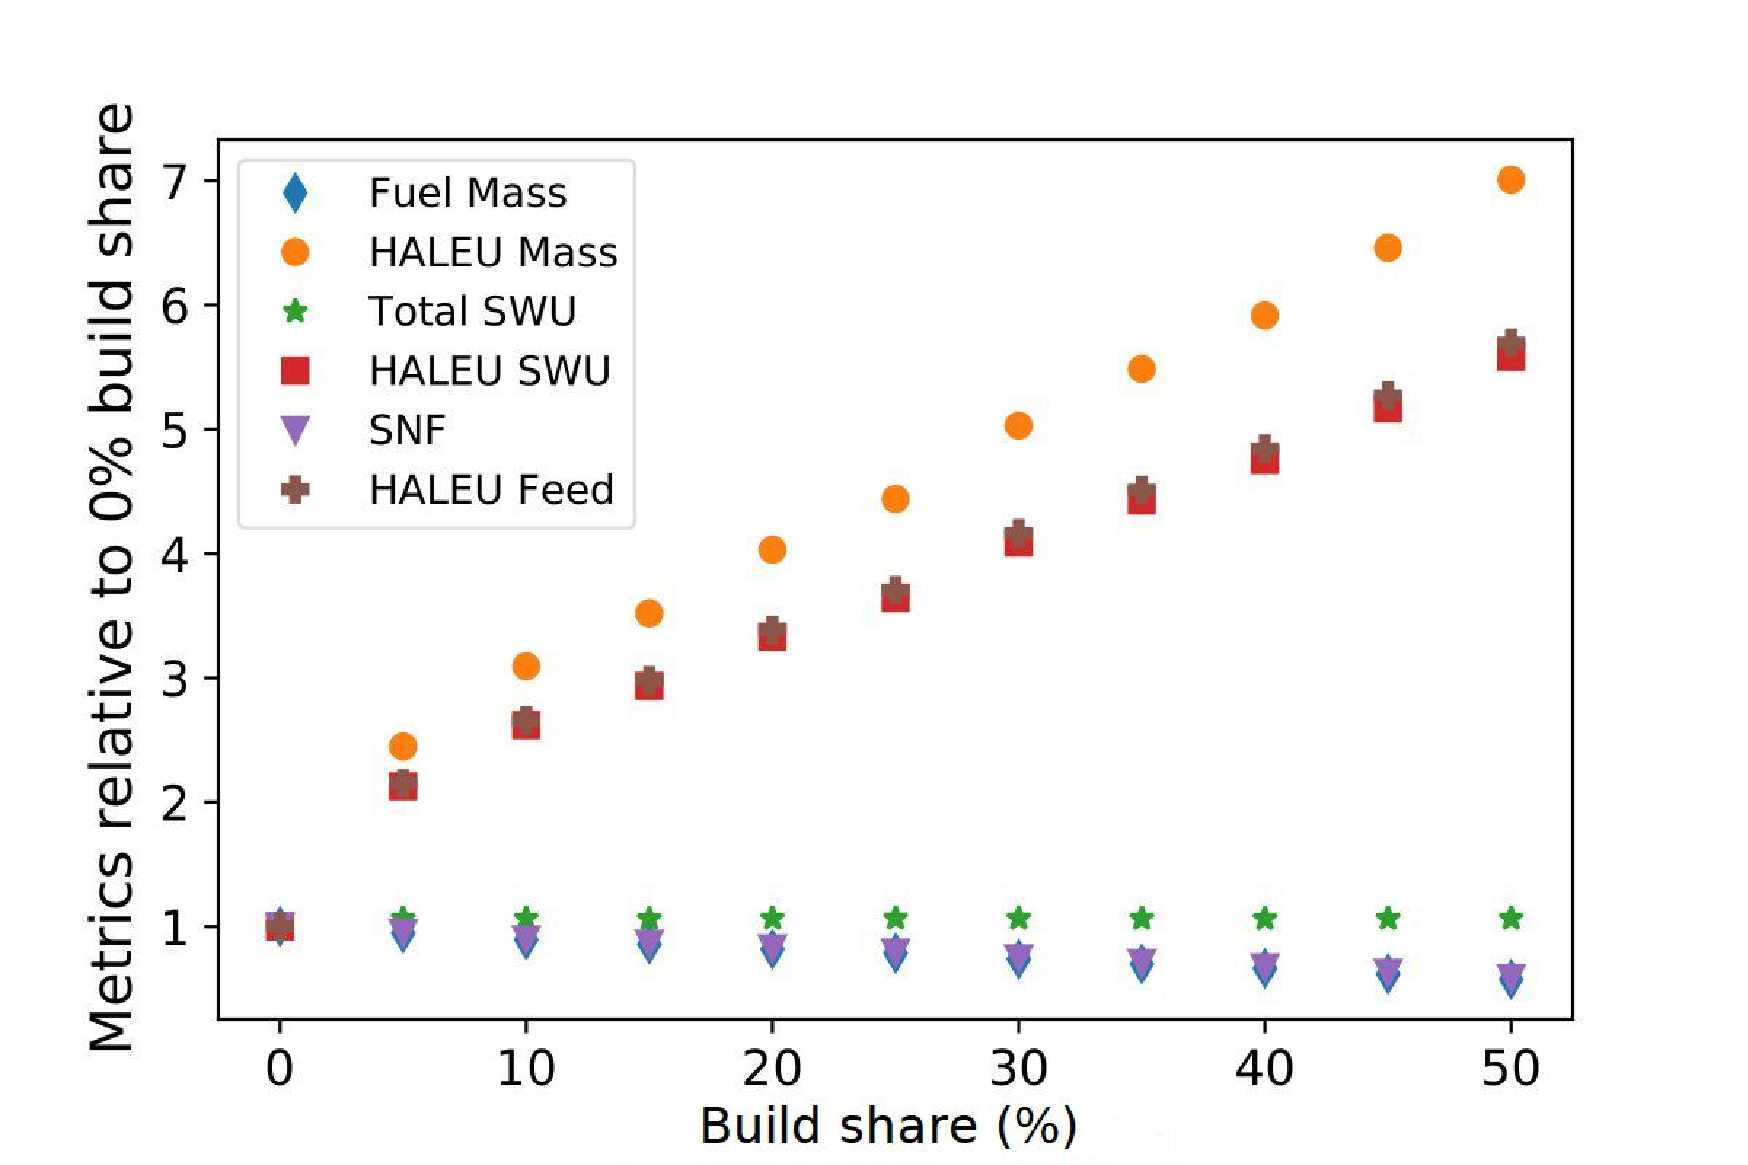
\includegraphics[scale=0.8]{xe100.pdf}
    \caption{Change in each metric as a function of Xe-100 build share, 
    relative to a build share of 0\%.}
    \label{fig:xe100_scenario7}
\end{figure}

\begin{figure}
    \centering
    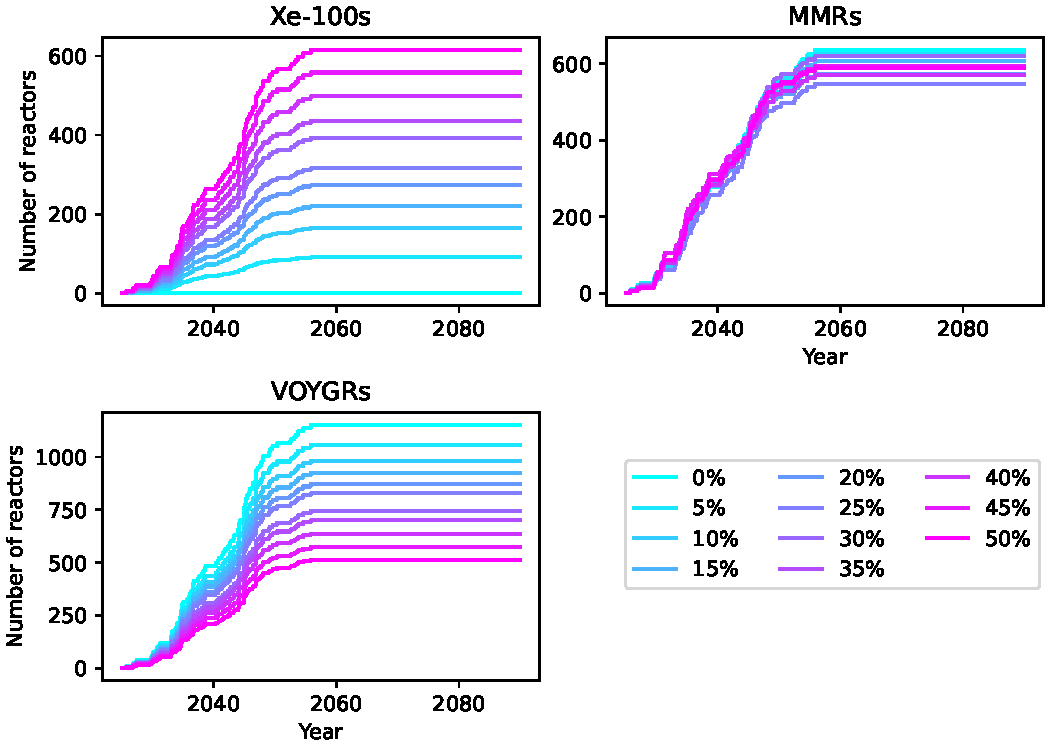
\includegraphics[scale=0.7]{xe100_combined_reactors.pdf}
    \caption{Number of Xe-100s (top left), MMRs (top right), and VOYGRs
    (bottom left) as a function of Xe-100 build share.}
    \label{fig:xe100_s7_combined_reactors}
\end{figure}

The \gls{HALEU}-related metrics increase with Xe-100 build share because more the 
power comes from advanced reactors requiring \gls{HALEU}. The total fuel mass and 
\gls{SNF} mass decrease because the Xe-100s are primarily replacing VOYGRs, and the 
Xe-100 requires less fuel per unit time and energy than the VOYGR, as discussed 
in Chapter \ref{ch:once_through_results}. The total \gls{SWU} capacity required 
is relatively constant, decreasing between 0.3-1.7\% compared to the \gls{SWU} capacity 
required for a 0\% Xe-100 build share. This stagnant behavior of the total 
\gls{SWU} capacity is consistent with the similar \gls{SWU} capacity required 
by Scenarios 3-7 in Section \ref{sec:nogrowth_swu}, when either the Xe-100 or 
VOYGR are primarily deployed. These results highlight the trade-off between the
\gls{HALEU}-related metrics and the total fuel mass and \gls{SNF} mass in deploying 
the Xe-100 versus the VOYGR. Both reactors require similar \gls{SWU} capacities, 
but because of the different product assays required the cascade configuration 
will vary. 

The \gls{HALEU}-related metrics increase to up to 538.2\% of the mass required 
for a 0\% Xe-100 build share. The total fuel mass and \gls{SNF} mass decrease 
to up to 44.11\% of the mass required for 1 0\% Xe-100 build share. 


\subsubsection{MMR build share}
As the \gls{MMR} build share increases all of the metrics increase, as shown 
in Figure \ref{fig:mmr_scenario7}. The total \gls{SWU}, \gls{HALEU} \gls{SWU}, 
and \gls{HALEU} feed have the greatest relative increase because more of the 
advanced reactor fleet uses the highest enrichment level of the three 
advanced reactors as the \gls{MMR} build share increases. The \gls{HALEU} mass 
increases with the \gls{MMR} build share because of the replacement of Xe-100s 
with \glspl{MMR} with increasing build share (see Figure \ref{fig:mmr_reactors_s7}).
The \gls{MMR} requires a greater fuel mass than the Xe-100, causing the increase 
in the \gls{HALEU} mass. The larger fuel mass required by the \gls{MMR}, compared 
with the Xe-100, compounds with the higher enrichment required by the \gls{MMR} 
to cause the greater relative increase in the total \gls{SWU}, \gls{HALEU} \gls{SWU}, 
and \gls{HALEU} feed. 

The \gls{SNF} mass does not experience the same 
relative increase as the total fuel mass because any fuel that is still in a 
reactor core at the end of the simulation is not accounted for in the 
\gls{SNF} mass. 
Based on the replacement of Xe-100s with \glspl{MMR} as the \gls{MMR} 
build share increases, these results highlight the effects of deploying the
\gls{MMR} over the Xe-100. 

\begin{figure}
    \centering
    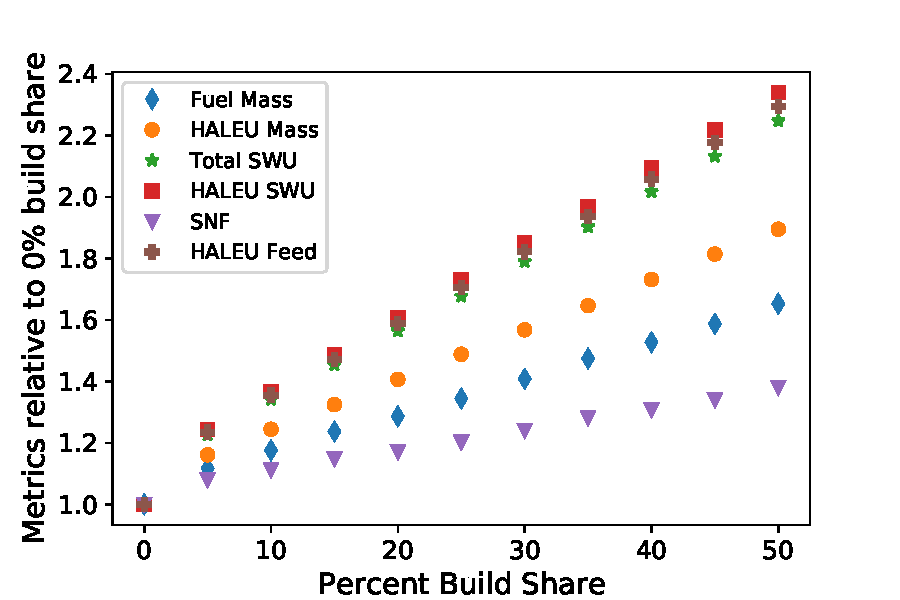
\includegraphics[scale=0.8]{mmr.pdf}
    \caption{Change in each metric as a function of MMR build share, 
    relative to a build share of 0\%.}
    \label{fig:mmr_scenario7}
\end{figure}


\begin{figure}
    \centering
    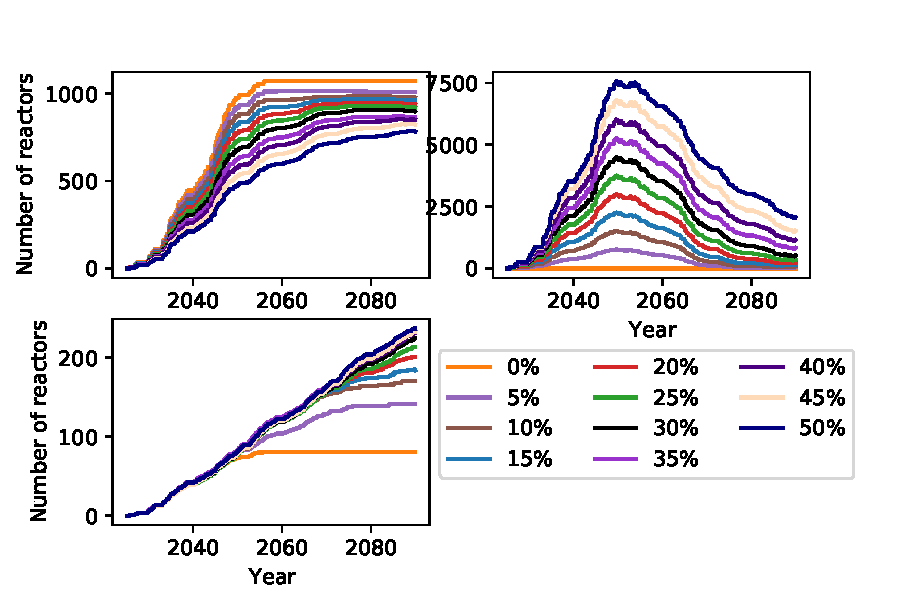
\includegraphics[scale=0.7]{mmr_combined_reactors.pdf}
    \caption{Number of Xe-100s (top left), MMRs (top right), and 
    VOYGRs (bottom left) deployed as a function of time and 
    MMR build share.}
    \label{fig:mmr_reactors_s7}
\end{figure}


\subsubsection{VOYGR build share}
When varying VOYGR build share, the impact on the metrics was 
opposite that of when varying the Xe-100 build share (Figure 
\ref{fig:voygr_scenario7}). The total fuel mass and \gls{SNF} mass 
increase, the \gls{HALEU}-related metrics decrease, and the total 
\gls{SWU} capacity remains relatively constant. This reversal 
of trends occurs because there is a replacement of Xe-100s with VOYGRs
with increasing build share (Figure \ref{fig:voygr_reactors_s7}), 
the opposite of what happens with an increasing Xe-100 build share. 

\begin{figure}
    \centering
    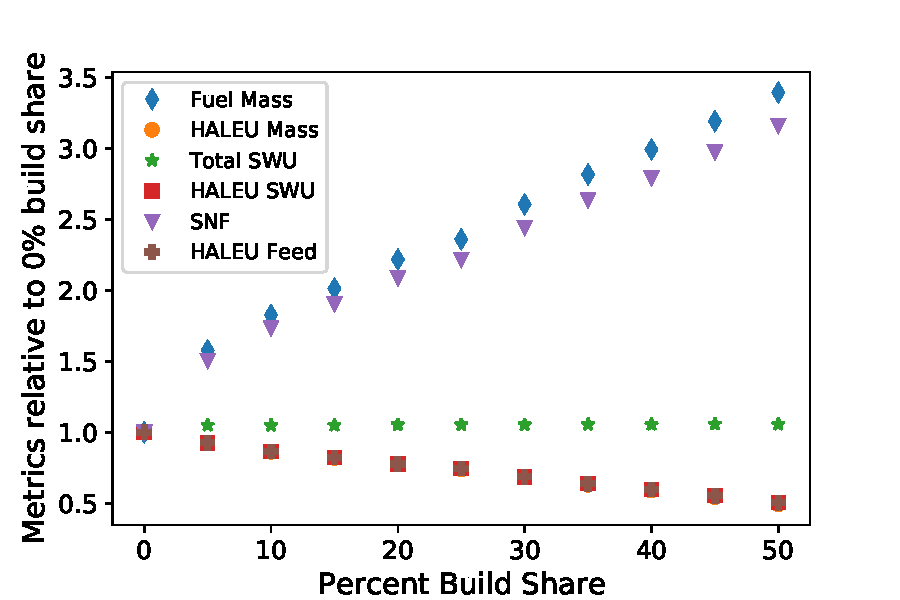
\includegraphics[scale=0.8]{voygr.pdf}
    \caption{Change in each metric as a function of VOYGR build share, 
    relative to a build share of 0\%.}
    \label{fig:voygr_scenario7}
\end{figure}

\begin{figure}
    \centering
    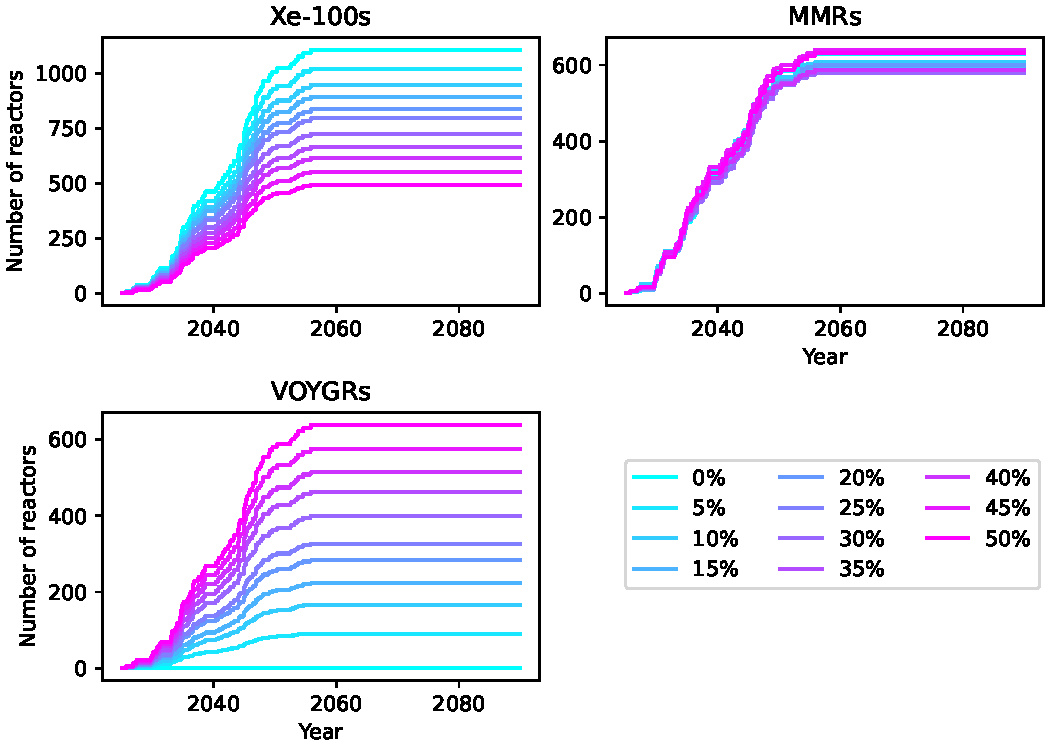
\includegraphics[scale=0.7]{voygr_combined_reactors.pdf}
    \caption{Number of Xe-100s (top left), MMRs (top right), and 
    VOYGRs (bottom left) deployed as a function of time and 
    VOYGR build share.}
    \label{fig:voygr_reactors_s7}
\end{figure}

The total \gls{SWU} capacity required varies between 99.6\%-101.2\% of the 
\gls{SWU} capacity needed for a 0\% VOYGR build share, a range of 1.077$\times 10^9$
- 1.092$\times 10^9$ kg-SWU (Table \ref{tab:oat_values}). The total fuel mass 
and \gls{SNF} mass increase 
up to 313.9\% of the mass required for a 0\% VOYGR build share, and the 
\gls{HALEU}-related metrics decrease to 49.77\% of the mass required 
for a 0\% VOYGR build share. The \gls{SNF} and total fuel masses increase 
because the VOYGR requires more fuel than the Xe-100, largely stemming from 
the difference in discharge burnup of these two reactors. The \gls{HALEU}-related 
metrics all decrease because the VOYGR does not require \gls{HALEU}, so as the 
VOYGR build share increases a smaller portion of the advanced reactor fleet 
requires \gls{HALEU}. While the trends from varying the VOYGR build share 
mirrors the trends from varying the Xe-100 build share, the magnitude of the 
changes are not the same. The magnitude difference occurs because these 
parameter variations cover adjacent but not overlapping design spaces. 

\subsubsection{Xe-100 burnup}
When varying the burnup of fuel discharged from Xe-100s, the metrics decrease 
as the burnup increases (Figure \ref{fig:xe100_bu_s7}). This decrease in material requirements because as 
the burnup is increased the fuel is going through the core more times or the 
length of each pass is longer. Therefore, the Xe-100s in the simulation are receiving 
less fuel at each refueling or receiving fuel less often as the burnup increases. 
Varying the burnup of the Xe-100 has a large impact on the metrics, up to fives times 
the material requirements compared with a burnup of 168 MWd/kgU, because most of 
the energy produced in these scenarios comes from Xe-100s and many more Xe-100s are 
deployed than \glspl{MMR} or VOYGRs. Therefore, changes to the Xe-100 refueling is 
magnified because of the greater number of the reactor deployed. 

\begin{figure}
    \centering
    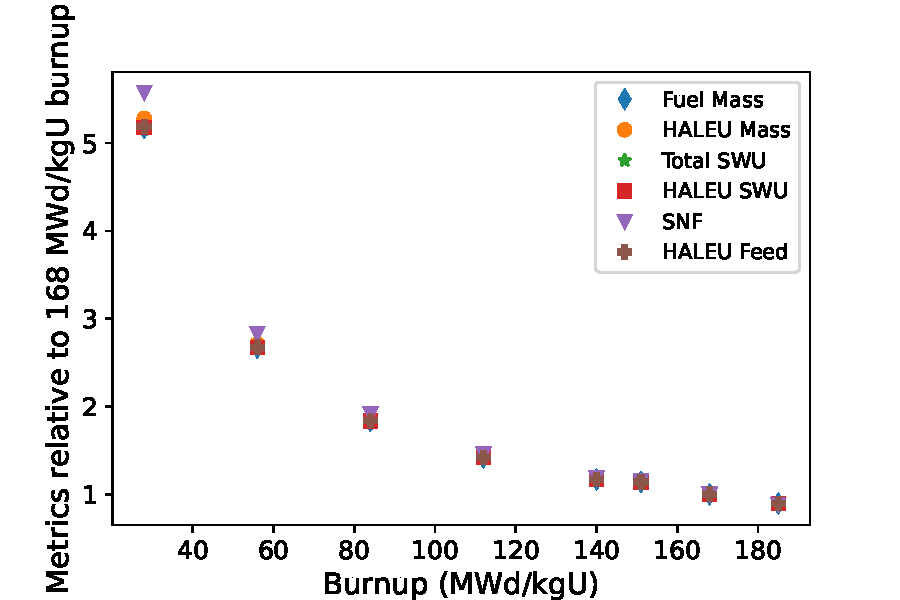
\includegraphics[scale=0.8]{xe100_bu.pdf}
    \caption{Change in metrics from varying the burnup of fuel 
    discharged from Xe-100, relative to a burnup of 168 MWd/kgU.}
    \label{fig:xe100_bu_s7}
\end{figure}

\subsubsection{MMR burnup}
When the \gls{MMR} discharge burnup is varied the metrics all decrease, similar 
to what was observed by varying the Xe-100 discharge burnup. One difference in 
the trends observed between varying these two parameters is the magnitude of 
the relative changes. Varying the \gls{MMR} burnup has a smaller relative effect 
on the metrics than varying the Xe-100 burnup because there are fewer \glspl{MMR} 
deployed in the transition. Therefore the impact on the cumulative metrics 
(what is reported here) is smaller. Another difference is that the total 
\gls{SWU}, \gls{HALEU} \gls{SWU}, and \gls{HALEU} feed increase the most 
when the \gls{MMR} burnup is low, compared with the \gls{SNF} having the 
greatest relative increase with the Xe-100 burnup is low. 

\begin{figure}
    \centering
    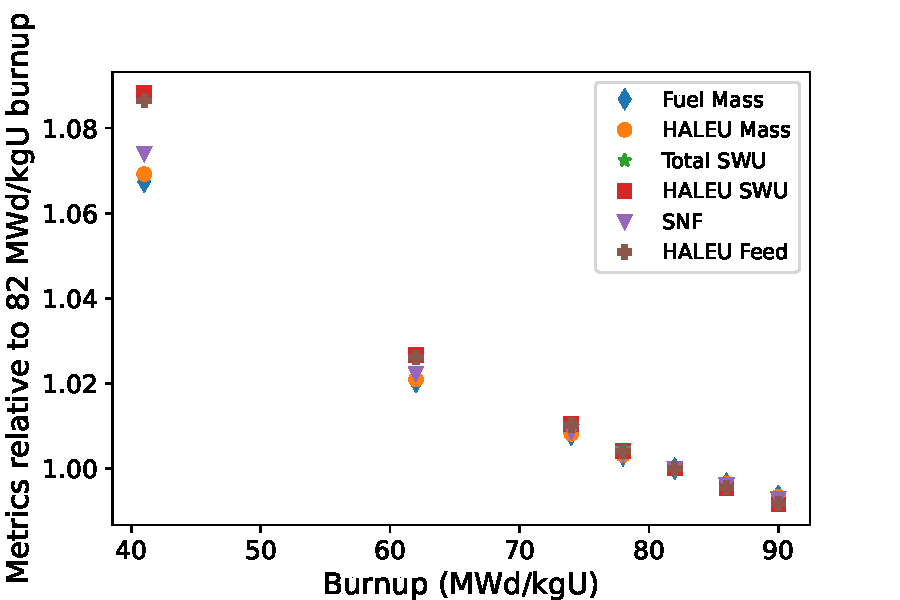
\includegraphics[scale=0.8]{mmr_bu.pdf}
    \caption{Change in metrics from varying the burnup of fuel 
    discharged from the MMR, relative to a burnup of 82 MWd/kgU.}
    \label{fig:mmr_bu_s7}
\end{figure}

\subsubsection{Burnup variations with a common build share}
To better investigate the effect of varying the discharge burnup of the Xe-100 
and \gls{MMR} without the influence of the deployment scheme preferentially
deploying Xe-100s, we repeated each set of analysis using a constant 20\% 
build share for both the Xe-100 and \gls{MMR} (VOYGRs met the remaining 60\%). 
Using a constant build share for 
both reactors means that they each will supply the same fraction of the energy demand.
However, because of the different power output for each reactor a constant build 
share does not mean that the same number of each reactor is built. 

Figure \ref{fig:bu_constant} shows the relative change in each metric as a result 
of varying the \gls{MMR} (Figure \ref{fig:mmr_bu_constant}) and Xe-100 
(Figure \ref{fig:xe100_bu_constant}) discharge burnup with the constant build 
share. Changing the \gls{MMR} burnup has a greater impact with the specified 20\% 
build share then when the build share was not specified. This change is because 
more \glspl{MMR} are deployed with a 20\% build share than when the build share is 
not specified. Conversely, the Xe-100 burnup has a smaller impact on the metrics 
with a 20\% build share than when a build share isn't specified because fewer 
Xe-100s are deployed. 

\begin{figure}
    \centering
    \begin{subfigure}{0.48\textwidth}
        \centering
        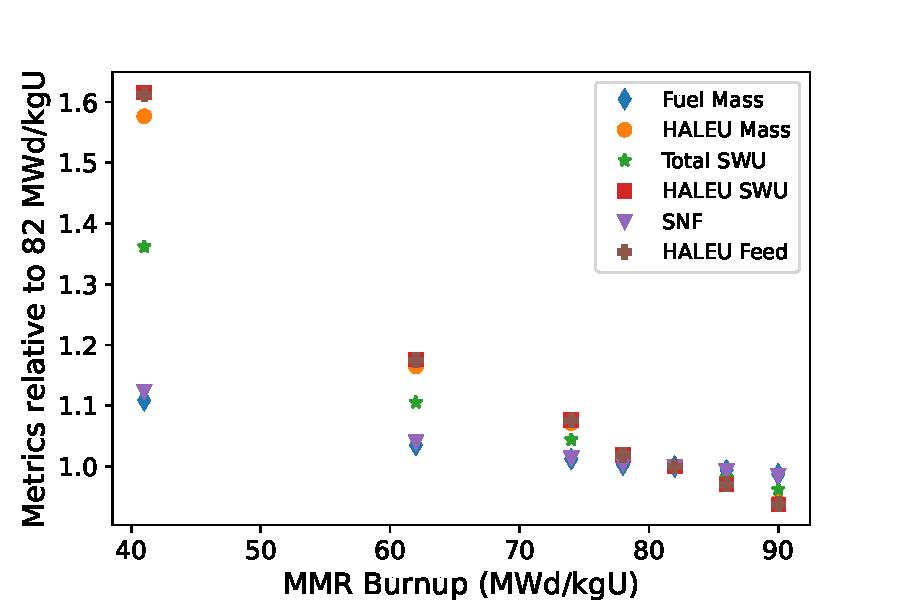
\includegraphics[width=\textwidth]{mmr_bu_constant.pdf}
        \caption{Change in metrics when varying the MMR discharge burnup, 
        assuming a constant 20\% build share for the MMR and Xe-100.}
        \label{fig:mmr_bu_constant}
    \end{subfigure}
    \hfill
    \begin{subfigure}{0.48\textwidth}
        \centering
        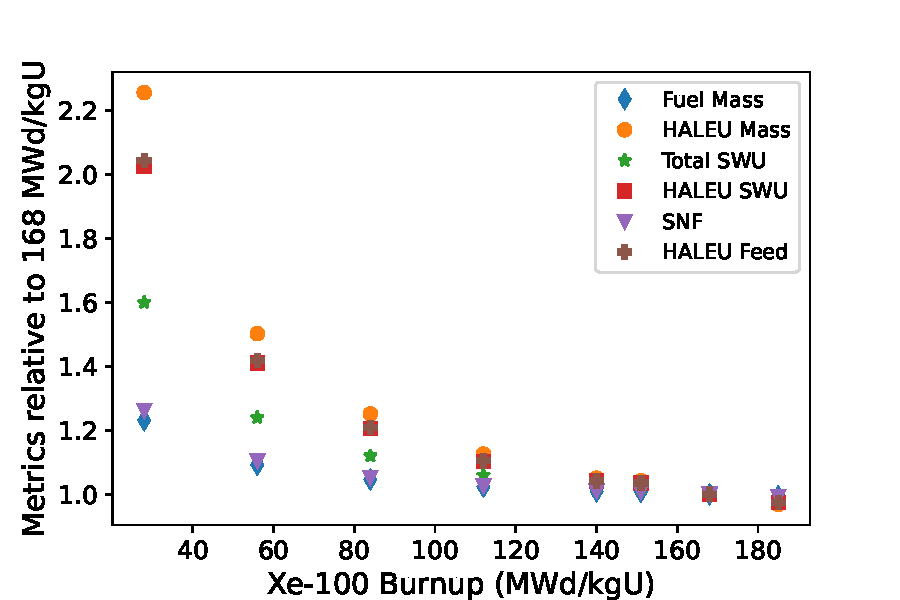
\includegraphics[width=\textwidth]{xe100_bu_constant.pdf}
        \caption{Change in metrics when varying the Xe-100 discharge burnup, 
        assuming a constant 20\% build share for the MMR and Xe-100.}
        \label{fig:xe100_bu_constant}
    \end{subfigure}
    \caption{Relative changes in the metrics caused by changes in the discharge 
    burnup of the HALEU-fueled advanced reactors, assuming a constant 
    20\% build share for the Xe-100 and MMR.}
    \label{fig:bu_constant}
\end{figure}

By applying a constant build share, variations in these parameters lead to 
more variation in the effect on the metrics than when a build share was not 
specified. In these scenarios, varying the discharge burnup of either reactor 
leads to the greatest impact on the \gls{HALEU}-related metrics while the  
total fuel mass and \gls{SNF} mass are affected the least. 
The \gls{HALEU}-related metrics are affected the most because most of the reactors 
in these scenarios are VOYGRs, which do not require \gls{HALEU}. Therefore, 
small increases in the each of the \gls{HALEU}-related metrics led to larger 
relative changes. Conversely, the total fuel mass and \gls{SNF} masses are 
affected less by changes in these parameters because the fuel and \gls{SNF} 
for the VOYGRs are constant and increase these values such that the changes 
observed cause a smaller relative change. 

\subsection{Scenario 14}